\documentclass[a4paper]{article}

\def\npart {III}
\def\nterm {Michaelmas}
\def\nyear {2017}
\def\nlecturer {A.\ G.\ Thomason}
\def\ncourse {Extremal Graph Theory}

% Imports
\ifx \nextra \undefined
  \usepackage[pdftex,
    hidelinks,
    pdfauthor={Dexter Chua},
    pdfsubject={Cambridge Maths Notes: Part \npart\ - \ncourse},
    pdftitle={Part \npart\ - \ncourse},
  pdfkeywords={Cambridge Mathematics Maths Math \npart\ \nterm\ \nyear\ \ncourse}]{hyperref}
  \title{Part \npart\ - \ncourse}
\else
  \usepackage[pdftex,
    hidelinks,
    pdfauthor={Dexter Chua},
    pdfsubject={Cambridge Maths Notes: Part \npart\ - \ncourse\ (\nextra)},
    pdftitle={Part \npart\ - \ncourse\ (\nextra)},
  pdfkeywords={Cambridge Mathematics Maths Math \npart\ \nterm\ \nyear\ \ncourse\ \nextra}]{hyperref}

  \title{Part \npart\ - \ncourse \\ {\Large \nextra}}
\fi

\author{Lectured by \nlecturer \\\small Notes taken by Dexter Chua}
\date{\nterm\ \nyear}

\usepackage{alltt}
\usepackage{amsfonts}
\usepackage{amsmath}
\usepackage{amssymb}
\usepackage{amsthm}
\usepackage{booktabs}
\usepackage{caption}
\usepackage{enumitem}
\usepackage{fancyhdr}
\usepackage{graphicx}
\usepackage{mathtools}
\usepackage{microtype}
\usepackage{multirow}
\usepackage{pdflscape}
\usepackage{pgfplots}
\usepackage{siunitx}
\usepackage{tabularx}
\usepackage{tikz}
\usepackage{tkz-euclide}
\usepackage[normalem]{ulem}
\usepackage[all]{xy}

\pgfplotsset{compat=1.12}

\pagestyle{fancyplain}
\lhead{\emph{\nouppercase{\leftmark}}}
\ifx \nextra \undefined
  \rhead{
    \ifnum\thepage=1
    \else
      \npart\ \ncourse
    \fi}
\else
  \rhead{
    \ifnum\thepage=1
    \else
      \npart\ \ncourse\ (\nextra)
    \fi}
\fi
\usetikzlibrary{arrows}
\usetikzlibrary{decorations.markings}
\usetikzlibrary{decorations.pathmorphing}
\usetikzlibrary{positioning}
\usetikzlibrary{fadings}
\usetikzlibrary{intersections}
\usetikzlibrary{cd}

\newcommand*{\Cdot}{\raisebox{-0.25ex}{\scalebox{1.5}{$\cdot$}}}
\newcommand {\pd}[2][ ]{
  \ifx #1 { }
    \frac{\partial}{\partial #2}
  \else
    \frac{\partial^{#1}}{\partial #2^{#1}}
  \fi
}

% Theorems
\theoremstyle{definition}
\newtheorem*{aim}{Aim}
\newtheorem*{axiom}{Axiom}
\newtheorem*{claim}{Claim}
\newtheorem*{cor}{Corollary}
\newtheorem*{defi}{Definition}
\newtheorem*{eg}{Example}
\newtheorem*{fact}{Fact}
\newtheorem*{law}{Law}
\newtheorem*{lemma}{Lemma}
\newtheorem*{notation}{Notation}
\newtheorem*{prop}{Proposition}
\newtheorem*{thm}{Theorem}

\renewcommand{\labelitemi}{--}
\renewcommand{\labelitemii}{$\circ$}
\renewcommand{\labelenumi}{(\roman{*})}

\let\stdsection\section
\renewcommand\section{\newpage\stdsection}

% Strike through
\def\st{\bgroup \ULdepth=-.55ex \ULset}

% Maths symbols
\newcommand{\bra}{\langle}
\newcommand{\ket}{\rangle}

\newcommand{\N}{\mathbb{N}}
\newcommand{\Z}{\mathbb{Z}}
\newcommand{\Q}{\mathbb{Q}}
\renewcommand{\H}{\mathbb{H}}
\newcommand{\R}{\mathbb{R}}
\newcommand{\C}{\mathbb{C}}
\newcommand{\Prob}{\mathbb{P}}
\renewcommand{\P}{\mathbb{P}}
\newcommand{\E}{\mathbb{E}}
\newcommand{\F}{\mathbb{F}}
\newcommand{\cU}{\mathcal{U}}
\newcommand{\RP}{\mathbb{RP}}
\newcommand{\CP}{\mathbb{CP}}

\newcommand{\ph}{\,\cdot\,}

\DeclareMathOperator{\sech}{sech}
\DeclareMathOperator{\cosech}{cosech}
\DeclareMathOperator{\cosec}{cosec}

\DeclareMathOperator{\covol}{covol}
\DeclareMathOperator{\vol}{vol}

\let\Im\relax
\let\Re\relax
\DeclareMathOperator{\Im}{Im}
\DeclareMathOperator{\Re}{Re}
\DeclareMathOperator{\im}{im}
\DeclareMathOperator{\image}{image}
\DeclareMathOperator{\Ann}{Ann}

\DeclareMathOperator*{\res}{res}
\DeclareMathOperator{\Res}{Res}
\DeclareMathOperator{\Ind}{Ind}

\DeclareMathOperator{\tr}{tr}
\DeclareMathOperator{\diag}{diag}
\DeclareMathOperator{\rank}{rank}
\DeclareMathOperator{\card}{card}
\DeclareMathOperator{\spn}{span}
\DeclareMathOperator{\adj}{adj}

\DeclareMathOperator{\erf}{erf}
\DeclareMathOperator{\erfc}{erfc}

\DeclareMathOperator{\ord}{ord}
\DeclareMathOperator{\Sym}{Sym}

\DeclareMathOperator{\sgn}{sgn}
\DeclareMathOperator{\orb}{orb}
\DeclareMathOperator{\stab}{stab}
\DeclareMathOperator{\ccl}{ccl}

\DeclareMathOperator{\lcm}{lcm}
\DeclareMathOperator{\hcf}{hcf}

\DeclareMathOperator{\Int}{Int}
\DeclareMathOperator{\id}{id}

\DeclareMathOperator{\betaD}{beta}
\DeclareMathOperator{\gammaD}{gamma}
\DeclareMathOperator{\Poisson}{Poisson}
\DeclareMathOperator{\binomial}{binomial}
\DeclareMathOperator{\multinomial}{multinomial}
\DeclareMathOperator{\Bernoulli}{Bernoulli}
\DeclareMathOperator{\like}{like}

\DeclareMathOperator{\var}{var}
\DeclareMathOperator{\cov}{cov}
\DeclareMathOperator{\bias}{bias}
\DeclareMathOperator{\mse}{mse}
\DeclareMathOperator{\corr}{corr}

\DeclareMathOperator{\otp}{otp}
\DeclareMathOperator{\dom}{dom}

\DeclareMathOperator{\Root}{Root}
\DeclareMathOperator{\supp}{supp}
\DeclareMathOperator{\rel}{rel}
\DeclareMathOperator{\Hom}{Hom}
\DeclareMathOperator{\Aut}{Aut}
\DeclareMathOperator{\Gal}{Gal}
\DeclareMathOperator{\Mat}{Mat}
\DeclareMathOperator{\End}{End}
\DeclareMathOperator{\Char}{char}
\DeclareMathOperator{\ev}{ev}
\DeclareMathOperator{\St}{St}
\DeclareMathOperator{\Lk}{Lk}
\DeclareMathOperator{\disc}{disc}
\DeclareMathOperator{\Isom}{Isom}
\DeclareMathOperator{\length}{length}
\DeclareMathOperator{\energy}{energy}
\DeclareMathOperator{\area}{area}
\DeclareMathOperator{\Syl}{Syl}
\DeclareMathOperator{\cl}{cl}
\DeclareMathOperator{\fix}{fix}

\newcommand{\GL}{\mathrm{GL}}
\newcommand{\SL}{\mathrm{SL}}
\newcommand{\PGL}{\mathrm{PGL}}
\newcommand{\PSL}{\mathrm{PSL}}
\newcommand{\PSU}{\mathrm{PSU}}
\newcommand{\Or}{\mathrm{O}}
\newcommand{\SO}{\mathrm{SO}}
\newcommand{\U}{\mathrm{U}}
\newcommand{\SU}{\mathrm{SU}}

\renewcommand{\d}{\mathrm{d}}
\newcommand{\D}{\mathrm{D}}

\tikzset{->/.style = {decoration={markings,
                                  mark=at position 1 with {\arrow[scale=2]{latex'}}},
                      postaction={decorate}}}
\tikzset{<-/.style = {decoration={markings,
                                  mark=at position 0 with {\arrowreversed[scale=2]{latex'}}},
                      postaction={decorate}}}
\tikzset{<->/.style = {decoration={markings,
                                   mark=at position 0 with {\arrowreversed[scale=2]{latex'}},
                                   mark=at position 1 with {\arrow[scale=2]{latex'}}},
                       postaction={decorate}}}
\tikzset{->-/.style = {decoration={markings,
                                   mark=at position #1 with {\arrow[scale=2]{latex'}}},
                       postaction={decorate}}}
\tikzset{-<-/.style = {decoration={markings,
                                   mark=at position #1 with {\arrowreversed[scale=2]{latex'}}},
                       postaction={decorate}}}

\tikzset{circ/.style = {fill, circle, inner sep = 0, minimum size = 3}}
\tikzset{mstate/.style={circle, draw, blue, text=black, minimum width=0.7cm}}

\definecolor{mblue}{rgb}{0.2, 0.3, 0.8}
\definecolor{morange}{rgb}{1, 0.5, 0}
\definecolor{mgreen}{rgb}{0.1, 0.4, 0.2}
\definecolor{mred}{rgb}{0.5, 0, 0}

\def\drawcirculararc(#1,#2)(#3,#4)(#5,#6){%
    \pgfmathsetmacro\cA{(#1*#1+#2*#2-#3*#3-#4*#4)/2}%
    \pgfmathsetmacro\cB{(#1*#1+#2*#2-#5*#5-#6*#6)/2}%
    \pgfmathsetmacro\cy{(\cB*(#1-#3)-\cA*(#1-#5))/%
                        ((#2-#6)*(#1-#3)-(#2-#4)*(#1-#5))}%
    \pgfmathsetmacro\cx{(\cA-\cy*(#2-#4))/(#1-#3)}%
    \pgfmathsetmacro\cr{sqrt((#1-\cx)*(#1-\cx)+(#2-\cy)*(#2-\cy))}%
    \pgfmathsetmacro\cA{atan2(#2-\cy,#1-\cx)}%
    \pgfmathsetmacro\cB{atan2(#6-\cy,#5-\cx)}%
    \pgfmathparse{\cB<\cA}%
    \ifnum\pgfmathresult=1
        \pgfmathsetmacro\cB{\cB+360}%
    \fi
    \draw (#1,#2) arc (\cA:\cB:\cr);%
}
\newcommand\getCoord[3]{\newdimen{#1}\newdimen{#2}\pgfextractx{#1}{\pgfpointanchor{#3}{center}}\pgfextracty{#2}{\pgfpointanchor{#3}{center}}}

\def\Xint#1{\mathchoice
   {\XXint\displaystyle\textstyle{#1}}%
   {\XXint\textstyle\scriptstyle{#1}}%
   {\XXint\scriptstyle\scriptscriptstyle{#1}}%
   {\XXint\scriptscriptstyle\scriptscriptstyle{#1}}%
   \!\int}
\def\XXint#1#2#3{{\setbox0=\hbox{$#1{#2#3}{\int}$}
     \vcenter{\hbox{$#2#3$}}\kern-.5\wd0}}
\def\ddashint{\Xint=}
\def\dashint{\Xint-}


\newcommand\ind{\mathrm{ind}}

\renewcommand\ex{\mathrm{ex}}
\begin{document}
\maketitle
{\small
\setlength{\parindent}{0em}
\setlength{\parskip}{1em}
Tur\'an's theorem, giving the maximum size of a graph that contains no complete $r$-vertex subgraph, is an example of an extremal graph theorem. Extremal graph theory is an umbrella title for the study of how graph and hypergraph properties depend on the values of parameters. This course builds on the material introduced in the Part II Graph Theory course, which includes Tur\'an's theorem and also the Erd\"os--Stone theorem.

The first few lectures will cover the Erd\"os--Stone theorem and stability. Then we shall treat Szemer\'edi's Regularity Lemma, with some applications, such as to hereditary properties. Subsequent material, depending on available time, might include: hypergraph extensions, the flag algebra method of Razborov, graph containers and applications.

\subsubsection*{Pre-requisites}
A knowledge of the basic concepts, techniques and results of graph theory, as afforded by the Part II Graph Theory course, will be assumed. This includes Tur\'an's theorem, Ramsey's theorem, Hall's theorem and so on, together with applications of elementary probability.
}
\tableofcontents

\section{The \texorpdfstring{Erd\"os--Stone}{Erdos--Stone} theorem}
The starting point of extremal graph theory is perhaps Tur\'an's theorem, which you hopefully learnt from the IID Graph Theory course. To state the theory, we need the following preliminary definition:
\begin{defi}[Tur\'an graph]\index{Tur\'an graph}
  The \emph{Tur\'an graph} \term{$T_r(n)$} is the complete $r$-partite graph on $n$ vertices with class sizes $\lfloor n/r\rfloor$ or $\lceil n/r\rceil$. We write $t_r(n)$ for the number of edges in $T_r(n)$.\index{$t_r(n)$}
\end{defi}

The theorem then says
\begin{thm}[Tur\'an's theorem]\index{Tur\'an's theorem}
  If $G$ is a graph with $|G| = n$, $e(G) \geq t_r(n)$ and $G \not \supseteq K_{r+1}$. Then $G = T_r(n)$.
\end{thm}
This is an example of an \emph{extremal theorem}. More generally, given a fixed graph $F$, we seek
\[
  \ex(n, F) = \max \{e(G): |G| = n, G \not\supseteq F\}.
\]
Tur\'an's theorem tells us $\ex(n, K_{r + 1}) = t_r(n)$. We cannot find a nice expression for the latter number, but we have
\[
  \ex(n, K_{r + 1}) = t_r(n) \approx \left(1 - \frac{1}{r}\right)\binom{n}{2}.
\]
Tur\'an's theorem is a rather special case. First of all, we actually know the exact value of $\ex(n, F)$. Moreover, there is a unique \term{extremal graph} realizing the bound. Both of these properties do not extend to other choices of $F$.

By definition, if $e(G) > \ex(n, K_{r + 1})$, then $G$ contains a $K_{r + 1}$. The Erd\"os--Stone theorem tells us that as long as $|G| = n$ is big enough, this condition implies $G$ contains a much larger graph than $K_{r + 1}$.

\begin{notation}\index{$K_r(t)$}
  We denote by $K_r(t)$ the complete $r$-partite graph with $t$ vertices in each class.
\end{notation}
So $K_r(1) = K_r$ and $K_r(t) = T_r(rt)$.

\begin{thm}[Erd\"os--Stone, 1946]\index{Erd\"os--Stone theorem}
  Let $r \geq 1$ be an integer and $\varepsilon > 0$. Then there exists $d = d(r, \varepsilon)$ and $n_0 = n_0(r, \varepsilon)$ such that if $|G| = n \geq n_0$ and
  \[
    e(G) \geq \left(1 - \frac{1}{r} + \varepsilon \right) \binom{n}{2},
  \]
  then $G \supseteq K_{r + 1}(t)$, where $t = \lfloor d \log n\rfloor$.
\end{thm}
Note that we can remove $n_0$ from the statement simply by reducing $d$, since for sufficiently small $d$, whenever $n < n_0$, we have $\lfloor d \log n\rfloor = 0$.

One corollary of the theorem, and a good way to think about the theorem is that given numbers $r, \varepsilon, t$, whenever $|G| = n$ is sufficiently large, the inequality $e(G) \geq \left(1 - \frac{1}{r} + \varepsilon\right) \binom{n}{2}$ implies $G \subseteq K_{r + 1}(t)$.

To prove the Erd\"os--Stone theorem, a natural strategy is to try to throw away vertices of small degree, and so that we can bound the \emph{minimal degree} of the graph instead of the total number of edges. We will make use of the following lemma to do so:
\begin{lemma}
  Let $c, \varepsilon > 0$. Then there exists $n_1 = n_1(c, \varepsilon)$ such that if $|G| = n \geq n_1$ and $e(G) \geq (c + \varepsilon) \binom{n}{2}$, then $G$ has a subgraph $H$ where $\delta(H) \geq c |H|$ and $|H| \geq \sqrt{\varepsilon} n$.
\end{lemma}

\begin{proof}
  The idea is that we can keep removing the vertex of smallest degree and then we must eventually get the $H$ we want. Suppose this doesn't gives us a suitable graph even after we've got $\sqrt{\varepsilon}n$ vertices left. That means we can find a sequence
  \[
    G = G_n \supseteq G_{n - 1} \supseteq G_{n - 2} \supseteq \cdots G_s,
  \]
  where $s = \lfloor \varepsilon^{1/2}n \rfloor$, $|G_j| = j$ and the vertex in $G_j \setminus G_{j - 1}$ has degree $< cj$ in $G_j$.

  We can then calculate
  \begin{align*}
    e(G_s) &> (c + \varepsilon) \binom{n}{2} - c \sum_{j = s + 1}^n j \\
    &= (c + \varepsilon) \binom{n}{2} - c \left\{\binom{n+1}{2} - \binom{s + 1}{2}\right\} \\
    &\sim \frac{\varepsilon n^2}{2}
  \end{align*}
  as $n$ gets large (since $c$ and $s$ are fixed numbers). In particular, this is $> \binom{s}{2}$. But $G_s$ only has $s$ vertices, so this is impossible.
\end{proof}

Using this, we can reduce the Erd\"os--Stone theorem to a version that talks about the minimum degree instead.
\begin{lemma}
  Let $r \geq 1$ be an integer and $\varepsilon > 0$. Then there exists a $d_1 = d_1(r, \varepsilon)$ and $n_2 = n_2(r, \varepsilon)$ such that if $|G| = n \geq n_2$ and
  \[
    \delta(G) \geq \left(1 - \frac{1}{r} + \varepsilon\right)n,
  \]
  then $G \supseteq K_{r + 1}(t)$, where $t = \lfloor d_1 \log n\rfloor$.
\end{lemma}
We first see how this implies the Erd\"os--Stone theorem:

\begin{proof}[Proof of Erd\"os--Stone theorem]
  Provided $n_0$ is large, say $n_0 > n_1\left(1 - \frac{1}{r} + \frac{\varepsilon}{2}, \frac{\varepsilon}{2}\right)$, we can apply the first lemma to $G$ to obtain a subgraph $H \subseteq G$ where $|H| > \sqrt{\frac{\varepsilon}{2}} n$, and $\delta(H) \geq \left(1 - \frac{1}{r} + \frac{\varepsilon}{2}\right) |H|$.

  We can then apply our final lemma as long as $\sqrt{\frac{\varepsilon}{2}} n$ is big enough, and obtain $K_{r + 1}(t) \subseteq H \subseteq G$, with $t > \left\lfloor d_1(r, \varepsilon/2) \log \left(\sqrt{\frac{\varepsilon}{2}} n\right)\right\rfloor$.
\end{proof}

We can now prove the lemma.

\begin{proof}[Proof of lemma]
  We proceed by induction on $r$. If $r = 0$ or $\varepsilon \geq \frac{1}{r}$, the theorem is trivial. Otherwise, by the induction hypothesis, we may assume $G \supseteq K_r(T)$ for
  \[
    T = \left\lfloor \frac{2t}{\varepsilon r}\right\rfloor.
  \]
  Call it $K = K_r(T)$. This is always possible, as long as
  \[
    d_1(r, \varepsilon) < \frac{\varepsilon r}{2} d_1\left(r - 1, \frac{1}{r(r - 1)}\right).
  \]
  The exact form is not important. The crucial part is that $\frac{1}{r(r - 1)} = \frac{1}{r - 1} - \frac{1}{r}$, which is how we chose the $\varepsilon$ to put into $d_1(r - 1, \varepsilon)$.

  Let $U$ be the set of vertices in $G - K$ having at least $\left(1 - \frac{1}{r} + \frac{\varepsilon}{2}\right)|K|$ neighbours in $K$. Calculating
  \[
    \left(1 - \frac{1}{r} + \frac{\varepsilon}{2}\right) |K| = \left(1 - \frac{1}{r} + \frac{\varepsilon}{2}\right) rT = (r - 1)T + \frac{\varepsilon r}{2}T \geq (r - 1)T + t,
  \]
  we see that every element in $U$ is joined to at least $t$ vertices in each class, and hence is joined to some $K_r(t) \subseteq K$.

  So we have to show that $|U|$ is large. If so, then by a pigeonhole principle argument, it follows that we can always find enough vertices in $U$ so that adding them to $K$ gives a $K_{r + 1}(t)$.
  \begin{claim}
    There is some $c > 0$ (depending on $r$ and $\varepsilon$) such that for $n$ sufficiently large, we have
    \[
      |U| \geq cn.
    \]
  \end{claim}

  The argument to establish these kinds of bounds is standard, and will be used repeatedly. We write $e(K, G - K)$ for the number of edges between $K$ and $G - K$. By the minimum degree condition, each vertex of $K$ sends at least $\left(1 - \frac{1}{r} + \varepsilon\right)n - |K|$ edges to $G - K$. Then we have two inequalities
  \begin{align*}
    |K| \left\{\left(1 - \frac{1}{r} + \varepsilon\right)n - |K|\right\} &\leq e(K, G - K) \\
    &\leq |U||K| + (n - |U|) \left(1 - \frac{1}{r} + \frac{\varepsilon}{2}\right)|K|.
  \end{align*}
  Rearranging, this tells us
  \[
    \frac{\varepsilon n}{2} - |K| \leq |U| \left(\frac{1}{r} - \frac{\varepsilon}{2}\right).
  \]
  Now note that $|K| \sim \log n$, so for large $n$, the second term on the left is negligible, and it follows that $U \sim n$.

  We now want to calculate the number of $K_r(t)$'s in $K$. To do so, we use the simple inequality
  \[
    \binom{n}{k} \leq \left(\frac{e n}{k}\right)^k.
  \]
  Then we have
  \[
    \# K_r(t) = \binom{T}{t}^r \leq \left(\frac{eT}{t}\right)^{rt} \leq \left(\frac{3e}{\varepsilon r}\right)^{rt} \leq \left(\frac{3e}{\varepsilon r}\right)^{rd\log n} = n^{rd \log (3e/\varepsilon r)}% \leq \frac{\varepsilon r n}{3t} \leq \frac{|U|}{t},
  \]
  Now if we pick $d$ sufficiently small, then this tells us $\#K_r(t)$ grows sublinearly with $n$. Since $|U|$ grows linearly, and $t$ grows logarithmically, it follows that for $n$ large enough, we have
  \[
    |U| \geq t\cdot \# K_r(t).
  \]
  Then by the pigeonhole principle, there must be a set $W \subseteq U$ of size $t$ joined to the same $K_r(t)$, giving a $K_{r + 1}(t)$.
\end{proof}

Erd\"os and Simonovits noticed that Erd\"os--Stone allows us to find $\ex(n, F)$ asymptotically for all $F$.

\begin{thm}[Erd\"os--Simonovits]
  Let $F$ be a fixed graph with chromatic number $\chi(F) = r + 1$. Then
  \[
    \lim_{n \to \infty} \frac{\ex(n, F)}{\binom{n}{2}} = 1 - \frac{1}{r}.
  \]
\end{thm}

\begin{proof}
  Since $\chi(F) = r + 1$, we know $F$ cannot be embedded in an $r$-partite graph. So in particular, $F \not\subseteq T_r(n)$. So
  \[
    \ex(n, F) \geq t_r(n) \geq \left(1 - \frac{1}{r}\right)\binom{n}{2}.
  \]
  On the other hand, given any $\varepsilon > 0$, if $|G| = n$ and
  \[
    e(G) \geq \left(1 - \frac{1}{r} + \varepsilon\right) \binom{n}{2},
  \]
  then by the Erd\"os--Stone theorem, we have $G \supseteq K_{r + 1}(|F|) \supseteq F$ provided $n$ is large. So we know that for every $\varepsilon > 0$, we have
  \[
    \limsup \frac{\ex(n, F)}{\binom{n}{2}} \leq 1 - \frac{1}{r} + \varepsilon.
  \]
  So we are done.
\end{proof}
If $r > 1$, then this gives us a genuine asymptotic expression for $\ex(n, F)$. However, if $r = 1$, i.e.\ $F$ is a bipartite graph, then this only tells us $\ex(n, F) = o\left(\binom{n}{2}\right)$, but doesn't tell us about the true asymptotic behaviour.

To end the chapter, we show that $t \sim \log n$ is indeed the best we can do in the Erd\"os--Stone theorem, by actually constructing some graphs.
\begin{thm}
  Given $r \in \N$, there exists $\varepsilon_r > 0$ such that if $0 < \varepsilon < \varepsilon_r$, then there exists $n_3(r, \varepsilon)$ so that if $n > n_3$, there exists a graph $G$ of order $n$ such that
  \[
    e(G) \geq \left(1 - \frac{1}{r} + \varepsilon\right) \binom{n}{2}
  \]
  but $K_{r + 1}(t) \not\subseteq G$, where
  \[
    t = \left\lceil \frac{3 \log n}{\log 1/\varepsilon}\right\rceil.
  \]
\end{thm}
So this tells us we cannot get better than $t \sim \log n$, and this gives us some bound on $d(r, \varepsilon)$.

\begin{proof}
  Start with the Tur\'an graph $T_r(n)$. Let $m = \left\lceil \frac{n}{r} \right\rceil$. Then there is a class $W$ of $T_r(n)$ of size $m$. The strategy is to add $\varepsilon \binom{n}{2}$ edges inside $W$ to obtain $G$ such that $G[W]$ (the subgraph of $G$ formed by $W$) does not contain a $K_2(t)$. It then follows that $G \not\supseteq K_{r + 1}(t)$, but also
  \[
    e(G) \geq t_r(n) + \varepsilon \binom{n}{2} \geq \left(1 - \frac{1}{r} +\varepsilon \right) \binom{n}{2},
  \]
  as desired.

  To see that such an addition is possible, we choose edges inside $W$ independently with probability $p$, to be determined later. Let $X$ be the number of edges chosen, and $Y$ be the number of $K_2(t)$ created. If $\E[X - Y] > \varepsilon \binom{n}{2}$, then this means there is an actual choice of edges with $X - Y > \varepsilon \binom{n}{2}$. We then remove an edge from each $K_2(t)$ to leave a $K_2(t)$-free graph with at least $X - Y > \varepsilon \binom{n}{2}$ edges.

  So we want to actually compute $\E[X - Y]$. Seeing that asymptotically, $m$ is much larger than $t$, we have
  \begin{align*}
    \E[X - Y] &= \E[X] - \E[Y] \\
    &= p\binom{m}{2} - \frac{1}{2}\binom{m}{t} \binom{m - t}{t} p^{t^2}\\
    &\sim \frac{1}{2} pm^2 - \frac{1}{2} m^{2t} p^{t^2}\\
    &= \frac{1}{2} pm^2 (1 - m^{2t - 2} p^{t^2 - 1})\\
    &= \frac{1}{2} pm^2 (1 - (m^2 p^{t + 1})^{t - 1}).
  \end{align*}
  We pick $p = 3 \varepsilon r^2$ and $\varepsilon_r = (3r^2)^{-6}$. Then $p < \varepsilon^{5/6}$, and
  \[
    m^2 p^{t + 1} < m^2 \varepsilon^{5/6 (t + 1)} < (m^2 m^{-5/2})^{t - 1} < \frac{1}{2}. % return to this
  \]
  Hence, we find that
  \[
    \E[x - y] \geq \frac{1}{4} p m^2 > \varepsilon \binom{n}{2}.
  \]
\end{proof}

Let's summarize what we have got so far. Let $t(n, r, \varepsilon)$ be the largest value of $t$ such that a graph of order $n$ with $\left(1 - \frac{1}{r} + \varepsilon \right) \binom{n}{2}$ edges is guaranteed to contain $K_{r + 1}(t)$. Then we know $t(n, r, \varepsilon)$ grows with $n$ like $\log n$. If we are keen, we can ask how $t$ depends on the other terms $r$ and $\varepsilon$. We just saw that
\[
  t(n, r, \varepsilon) \leq \frac{3 \log n}{\log 1/\varepsilon}.
\]
So we see that the dependence on $\varepsilon$ is at most logarithmic, and in 1976, Bollob\'as, Erd\"os and Simonovits showed that
\[
  t(n, r, \varepsilon) \geq c \frac{\log n}{r \log 1/\varepsilon}
\]
for some $c$. Thus, $t(n, r, \varepsilon)$ also grows (inverse) logarithmically with $\varepsilon$.

In our original bound, there is no dependence on $r$, which is curious. While Bollob\'as, Erd\"os and Simonovits's bound does, in 1978, Chv\'atal and Szemer\'edi showed that
\[
  t \geq \frac{1}{500} \frac{\log n}{\log 1/\varepsilon}
\]
if $n$ is large. So we know there actually is no dependence on $r$.

We can also ask about the containment of less regular graphs than $K_r(t)$. In 1994, Bollob\'as and Kohayakawa adapted the proof of the Erd\"os--Stone theorem to show that there is a constant $c$ such that for any $0 < \gamma < 1$, if $e(G) \geq \left(1 - \frac{1}{r} + \varepsilon\right) \binom{n}{2}$ and $n$ is large, then we can find a complete $(r + 1)$-partite subgraph with class sizes
\[
  \left\lfloor c \gamma \frac{\log n}{r \log 1/\varepsilon}\right\rfloor, \left\lfloor c \gamma \frac{\log n}{\log r}\right\rfloor, r - 1\text{ times}, \left\lfloor c \varepsilon^{\frac{3}{2} - \frac{\gamma}{2}} n^{1 - \gamma}\right\rfloor.
\]
We might wonder if we can make similar statements for hypergraphs. It turns out all the analogous questions are open. Somehow graphs are much easier.

\section{Stability}
An extremal problem is \term{stable} if every near-optimal extremal example looks close to some optimal (unique) example. Stability pertain for $\ex(n, F)$.

\begin{thm}
  Let $t, r \geq 2$ be fixed, and suppose $|G| = n$ and $G \not\supseteq K_{r + 1}(t)$. If
  \[
    e(G) = \left(1 - \frac{1}{r} + o(1)\right) \binom{n}{2}.
  \]
  Then
  \begin{enumerate}
    \item There exists $T_r(n)$ on $V(G)$ with $|E(G) \Delta E(T_r(n))| = o(n^2)$.
    \item $G$ contains an $r$-partite subgraph with $\left(1 - \frac{1}{r} + o(1)\right) \binom{n}{2}$ edges.
    \item $G$ contains an $r$-partite subgraph with minimum degree $\left(1 - \frac{1}{r} + o(1)\right)n$.
  \end{enumerate}
\end{thm}

The outline of the proof is as follows: we first show that the three statements are equivalent, so that we only have to prove (ii). To prove (ii), we first use Erd\"os--Stone to find some $K_r(s)$ living inside $G$ (for some $s$), which is a good $r$-partite subgraph of $G$, but with not quite the right number of vertices. We now look at the remaining vertices. For each vertex $v$, find the $C_i$ such that $v$ is connected to as few vertices in $C_i$ as possible, and enlarge $C_i$ to include that as well. After doing this, $C_i$ will have quite a few edges between its vertices, and we throw those away. The hope is that there are only $o(n^2)$ edges to throw away, so that we still have $\left(1 - \frac{1}{r} + o(1)\right) \binom{n}{2}$ edges left. It turns out as long as we throw out some ``bad'' vertices, we will be fine.

\begin{proof}
  We first prove (ii), which looks the weakest. We will then argue that the others follow from this (and in fact they are equivalent).

  By Erd\"os--Stone, we can always find some $K_r(s) = K \subseteq G$ for some $s = s(n) \to \infty$. We can, of course, always choose $s(n)$ so that $s(n) \leq \log n$, which will be helpful for our future analysis. We let $C_i$ be the $i$th class of $K$.

  \begin{itemize}
    \item By throwing away $o(n)$ vertices, we may assume that
      \[
        \delta(G) \geq \left(1 - \frac{1}{r} + o(1)\right) n
      \]
    \item Let $X$ be the set of all vertices joined to at least $t$ vertices in each $C_i$. Note that there are $\binom{s}{t}^r$ many copies of $K_r(t)$'s in $K$. So by the pigeonhole principle, we must have $|X| < t \binom{s}{t}^r = o(n)$, or else we can construct a $K_{r + 1}(t)$ inside $G$.
    \item Let $Y$ be the set of vertices joined to fewer than $(r - 1) s - \frac{s}{2t} + t$ other vertices. By our bound on $\delta(G)$, we certainly have
      \[
        e(K, G - K) \geq s(r - 1 + o(1))n.
      \]
      On the other hand, every element of $G$ is certainly joined to at most $(r-1)s + t$ edges, since $X$ was thrown away. So we have
      \[
        ((r - 1)s + t)(n - |Y|) + |Y| \left((r - 1) s - \frac{s}{2t} + t\right) \geq e(K, G - K).
      \]
      So we deduce that $|Y| = o(n)$. Throw $Y$ away.
  \end{itemize}
  Let $V_i$ be the set of vertices in $G \setminus K$ joined to fewer than $t$ of $C_i$. It is now enough to show that $e(G[V_i]) = o(n^2)$. We can then throw away the edges in each $V_i$ to obtain an $r$-partite graph.

  Suppose on the contrary that $e(G[V_j]) \geq \varepsilon n^2$, say, for some $j$. Then Erd\"os--Stone with $r = 1$ says we have $G[V_j] \supseteq K_2(t)$. Each vertex of $K_2(t)$ has at least $s - \frac{s}{2t} + 1$ in each other $C_i$, for $i \not= j$. So we see that $K_2(t)$ has at least $s - 2t \left(\frac{s}{2t} - 1\right) > t$ common neighbours in each $C_i$, giving $K_{r + 1}(t) \subseteq G$.

  It now remains to show that (i) and (iii) follows from (ii). The details are left for the example sheet, but we sketch out the rough argument. (ii) $\Rightarrow$ (i) is straightforward, since an $r$-partite graph with that many edges is already pretty close to being a Tur\'an graph.

  To deduce (iii), since we can assume $\delta(G) \geq \left(1 - \frac{1}{r} + o(1)\right) n$, we note that if (iii) did not hold, then we have $\varepsilon n$ vertices of degree $\leq \left(1 - \frac{1}{r} - \varepsilon\right)n$, and their removal leaves a graph of order $(1 - \varepsilon) n$ with at least
  \[
    \left(1 - \frac{1}{r} + o(1)\right)\binom{n}{2} - \varepsilon n \left(1 - \frac{1}{r} - \varepsilon\right)n > \left(1 - \frac{1}{r} + \varepsilon^2\right) \binom{(1 - \varepsilon)n}{2},
  \]
  which by Erd\"os--Stone would contain $K_{r + 1}(t)$. So we are done.
\end{proof}
%if we want this to succeed, we have to throw out some ``bad'' vertices before we start.
%
%\begin{proof}
%  Clearly $(i) \Rightarrow (ii)$, and also $(ii) \Rightarrow (i)$, since an $r$-partite graph with that many edges is already pretty close to a Tur\'an graph. This is made precise on the example sheet.
%
%  It is also easy to see that $(iii) \Rightarrow (ii)$. Note too that we may jettison $o(n)$ vertices if we wish to. By doing that, we may assume that $\delta(G) \geq \left(1 - \frac{1}{r} + o(1)\right) n$. So $(ii) \Rightarrow (iii)$, for otherwise we have $\varepsilon n$ vertices of degree $\leq \left(1 - \frac{1}{r} - \varepsilon\right)n$, and their removal leaves a graph of order $(1 - \varepsilon) n$ with at least
%  \[
%    \left(1 - \frac{1}{r} + o(1)\right)\binom{n}{2} - \varepsilon n \left(1 - \frac{1}{r} - \varepsilon\right)n > \left(1 - \frac{1}{r} + \varepsilon^2\right) \binom{(1 - \varepsilon)n}{2},
%  \]
%  which by Erd\"os--Stone would contain $K_{r + 1}(t)$.
%
%  So our three properties can be assumed to be equivalent, and (ii) is the weakest-looking statement. So we will prove $(ii)$
%
%  Now we have $G \supseteq K = K_r(s)$ where $\log n \geq s = s(n) \to \infty$ by Erd\"os--Stone. Let $C_i$ be the $i$th class of $K$. Let $X$ be the set of vertices joined to at least $T$ in each $C_i$. There are $\binom{s}{t}^{r}$ many $K_r(t)$'s in $K$, and since $G \supseteq K_{r + 1}(t)$, we have $|X| < t \binom{s}{t}^r = o(n)$. Jettison $X$.
%
%  Let $Y$ be the set of vertices joined to fewer than $(r - 1)S - \frac{s}{2t} + t$. Since $\delta(G) = \left(1 - \frac{1}{r} + o(1) \right) n$, we see
%  \[
%    e(K, G - K) \geq s(r - 1 + o(1))n.
%  \]
%  On the other hand, because $X$ has been jettisoned, we know
%  \[
%    ((r - 1)s + t)(n - |Y|) + |Y| \left((r - 1) s - \frac{s}{2t} + t\right) \geq e(K, G - K).
%  \]
%  So $|Y| = o(n)$. So we jettison $Y$.
%
%  The remaining vertices are partitioned by letting $V_i$ be the set of vertices in $G - K$ joined to fewer than $t$ of $C_i$. Now it is enough to show that $e(G[V_i]) = o(n^2)$, since then $V_1, \ldots, V_r$ are the classes of our $r$-partite subgraph.
%
%  Suppose on the contrary that $e(G[V_j]) \geq \varepsilon n^2$, say, for some $j$. Then Erd\"os--Stone with $r = 1$ says we have $G[V_j] \supseteq K_2(t)$. Each vertex of $K_2(t)$ has at least $s - \frac{s}{2t} + 1$ in each other $C_i$, for $i \not= j$. So we see that $K_2(t)$ has at least $s - 2t \left(\frac{s}{2t} - 1\right) > t$ common neighbours in each $C_i$, giving $K_{r + 1}(t) \subseteq G$.
%\end{proof}

\begin{cor}
  Let $\chi(F) = r + 1$, and let $G$ be extremal for $F$, i.e.\ $G \not\supseteq F$ and $e(G) = \ex(|G|, F)$. Then $\delta(G) = \left(1 - \frac{1}{r} + o(1)\right)n$.
\end{cor}

\begin{proof}
  By our asymptotic bound on $\ex(n, F)$, it cannot be that $\delta(G)$ is greater than $\left(1 - \frac{1}{r} + o(1)\right)n$. So there must be a vertex $v \in G$ with $d(v) \leq \left(1 - \frac{1}{r} - \varepsilon\right) n$.

  We now apply version (iii) of the stability theorem to obtain an $r$-partite subgraph $H$ of $G$. We can certainly pick $|F|$ vertices in the same part of $H$, which are joined to $m = \left(1 - \frac{1}{r} + o(1)\right)$ common neighbours. Form $G^*$ from $G - v$ by adding a new vertex $u$ joined to these $m$ vertices. Then $e(G^*) > e(G)$, and so the maximality of $G$ entails $G^* \supseteq F$.

  Pick a copy of $F$ in $G^*$. This must involve $u$, since $G$, and hence $G - v$ does not contain a copy of $F$. Thus, there must be some $x$ amongst the $|F|$ vertices mentioned. But then we can replace $u$ with $x$ and we are done.
\end{proof}

Sometimes, stability and bootstrapping can give exact results.

\begin{eg}
  $\ex(n, C_5) = t_2(n)$. In fact, $\ex(n, C_{2k + 1}) = t_2(n)$ if $n$ is large enough.
\end{eg}

\begin{thm}[Simonovits]
  Let $F$ be $(r + 1)$-edge-critical\index{$r$-edge-critical}, i.e.\ $\chi(F) = r + 1$ but $\chi(F) \setminus e) = r$ for every edge $e$ of $F$. Then for large $n$,
  \[
    \ex(n, F) = t_r(n).
  \]
  and the only extremal graph is $T_r(n)$.
\end{thm}
So we get a theorem like Tur\'an's theorem for large $n$.

\begin{proof}
  Let $G$ be an extremal graph for $F$ and let $H$ be an $r$-partite subgraph with
  \[
    \delta(H) = \left(1 - \frac{1}{r} + o(1)\right)n.
  \]
  Note that $H$ necessarily have $r$ parts of size $\left(\frac{1}{r} + o(1)\right)n$ each. Assign each of the $o(n)$ vertices in $V(G) \setminus V(H)$ to a class where it has fewest neighbours.

  Suppose some vertex $v$ has $\varepsilon n$ neighbours in its own class. Then it has $\geq \varepsilon n$ in each class. Pick $\varepsilon n$ neighbours of $v$ in each class of $H$. These neighbours span a graph with at least $\left(1 -\frac{1}{r} + o(1)\right) \binom{r\varepsilon n}{2}$ edges. So by Erd\"os--Stone (or arguing directly), they span $F - w$ for some vertex $w$ (contained in $K_r(|F|)$). Hence $G \supseteq F$, contradiction.

  Thus, each vertex of $G$ has only $o(n)$ vertices in its own class. So it is joined to all but $o(n)$ vertices in every other class.

  Suppose some class of $G$ contains an edge $xy$. Pick a set $Z$ of $|F|$ vertices in that class with $\{x, y\} \in Z$. Now $Z$ has $\left(\frac{1}{r} + o(1)\right)n$ common neighbours in each class, so (by Erd\"os--Stone or directly) these common neighbours span a $K_{r - 1}(|F|)$. But together with $Z$, we have a $K_r(|F|)$ but with an edge added inside a class. But by our condition that $F \setminus e$ is $r$-partite for any $e$, this subgraph contains an $F$. This is a contradiction.

  So we conclude that no class of $G$ contains an edge. So $G$ itself is $r$-partite, but the $r$-partite graph with most edges is $T_r(n)$, which does not contain $F$. So $G = T_r(n)$.
\end{proof}

\section{Supersaturation}
Supersaturation is about how many copies of $F$ must exist in a graph $G$ with $e(G) > \ex(n, F)$. Recall that an $\ell$-uniform hypergraph is a pair $(V, E)$, where $E \subseteq V^{(\ell)}$. We can define the extremal function of a class of hypergraphs $\mathcal{F}$ by
\[
  \ex(n, \mathcal{F}) = \max \{e(G): |G| = n, \text{$G$ contains no $f \in \mathcal{F}$}\}.
\]
Again we are interested in the limiting density
\[
  \pi(\mathcal{F}) = \lim_{n \to \infty} \frac{\ex(n, \mathcal{F})}{\binom{n}{\ell}}.
\]
It is an easy exercise to show that this limit always exists. We solved it explicitly for graphs explicitly previously, but we don't really need the Erd\"os--Stone theorem just to show that the limit exists.

The basic theorem in supersaturation is
\begin{thm}[Erd\"os--Simonovits]
  Let $H$ be some $\ell$-uniform hypergraph. Then for all $\varepsilon > 0$, there exists $\delta(H, \varepsilon)$ such that every $\ell$-uniform hypergraph $G$ with $|G| = n$ and
  \[
    e(G) > (\pi(H) + \varepsilon) \binom{n}{\ell}
  \]
  contains $\lfloor \delta n^{|H|}\rfloor$ copies of $H$.
\end{thm}
Note that $n^{|H|}$ is approximately the number of ways to choose $|H|$ vertices from $n$, so it's the number of possible candidates for subgraphs $H$.

\begin{proof}
  For each $m$-set $M \subseteq V(G)$, we let $G[M]$ be the sub-hypergraph induced by these vertices. If there are $\eta \binom{n}{m}$ subsets $M$ with $e(G[M]) > \left(\pi(H) + \frac{\varepsilon}{2}\right) \binom{m}{\ell}$, then
  \[
    \left(\pi(H) + \varepsilon\right) \binom{n}{\ell} \leq e(G) = \frac{\sum_M e(G[M])}{\binom{n - \ell}{m - \ell}} \leq \eta \frac{\binom{n}{m} \binom{m}{\ell} + (1 - \eta) \binom{n}{m} \left(\pi(H) + \frac{\varepsilon}{2}\right) \binom{m}{\ell}}{\binom{n - \ell}{m - \ell}}.
  \]
  So if $n > m$, then
  \[
    \pi(H) + \varepsilon \leq \eta + (1 + \eta) \left(\pi(H) + \frac{\varepsilon}{2}\right).
  \]
  So
  \[
    \eta \geq \frac{\frac{\varepsilon}{2}}{1 - \pi(H) - \frac{\varepsilon}{2}} > 0.
  \]
  The point is that it is positive, and that's all we care about.

  We pick $m$ large enough so that
  \[
    \ex(m, H) < \left(\pi(H) + \frac{\varepsilon}{2}\right) \binom{m}{\ell}.
  \]
  Then $H \subseteq G[M]$ for at least $\eta \binom{n}{m}$ choices of $M$. Hence $G$ contains at least
  \[
    \frac{\eta\binom{n}{m}}{\binom{n - |H|}{m - |H|}} = \frac{\eta\binom{n}{|H|}}{\binom{m}{|H|}},
  \]
  copies of $H$, and we are done. (Our results hold when $n$ is large enough, but we can choose $\delta$ small enough so that $\delta n^{|H|} < 1$ when $n$ is small)
\end{proof}

Let $k_P(G)$ be the number of copies of $K_p$ in $G$. Ramsey's theorem tells us $k_p(G) + k_p(\bar{G}) > 0$ if $|G|$ is large (where $\bar{G}$ is the complement of $G$). In the simplest case where $p = 3$, it turns out we can count these monochromatic triangles.
\begin{thm}[Lorden, 1961]
  Let $G$ have degree sequence $d_1, \ldots, d_n$. Then
  \[
    k_3(G) + k_3(\bar{G}) = \binom{n}{3} - (n - 2) e(G) + \sum_{i = 1}^n \binom{d_i}{2}.
  \]
\end{thm}

\begin{proof}
  The number of paths of length $2$ in $G$ and $\bar{G}$ is precisely
  \[
    \sum_{i = 1}^n \left(\binom{d_i}{2} + \binom{n - 1 - d_i}{2}\right) = 2 \sum_{i = 1}^n \binom{d_i}{2} - 2 (n - 2) e(G) + 3 \binom{n}{3}.
  \]
  since to find a path of length $2$, we pick the middle vertex and then pick the two edges. A complete or empty $K_3$ contains $3$ such paths; Other sets of three vertices contain exactly 1 such path. Hence
  \[
    \binom{n}{3} + 2 (k_3(G) + k_3(\bar{G}) = \text{number of paths of length $2$}.
  \]
\end{proof}
\begin{cor}[Goodman, 1959]
  We have
  \[
    k_3(G) + k_3(\bar{G}) \geq \frac{1}{24} n(n - 1)(n - 5).
  \]
\end{cor}

In particular, the Ramsey number of a triangle is at most $6$.

\begin{proof}
  Let $m = e(G)$. Then
  \[
    k_3(G) + k_3(\bar{G}) \geq \binom{n}{3} - (n - 2) m + n \binom{2m/n}{2}. % Cauchy--Schwarz
  \]
  Then minimize over $m$.
\end{proof}

This shows the minimum density of a monochromatic $K_3$ in a red/blue colouring of $K_n$ (for $n$ large) is $\sim \frac{1}{4}$. But if we colour edges monochromatic, then $\frac{1}{4}$ is the probability of having a triangle being monochromatic. So the density is achieved by a ``random colouring''. Recall also that the best bounds on the Ramsey numbers we have are obtained by random colourings. So we might think the best way of colouring if we want to minimize the number of monochromatic cliques is to do so randomly. However, this is not true. While we do not know what the minimum density of monochromatic $K_4$ in a red/blue colouring of $K_n$, it is already known to be $\frac{1}{33}$ (while $\frac{1}{32}$ is what we expect from a random colouring). It is also known by flag algebras to be $> \frac{1}{35}$. So we are not very far.

\begin{cor}
  For $m = e(G)$ and $n = |G|$, we have
  \[
    k_3(G) \geq \frac{m}{3n}(4m - n^2).
  \]
\end{cor}

\begin{proof}
  By Lorden's theorem, we know
  \[
    k_3(G) + k_3(\bar{G}) = \binom{n}{3} - (n - 2) e(\bar{G}) + \sum\binom{\bar{d}_i}{2},
  \]
  where $\bar{d}_i$ is the degree sequence in $\bar{G}$. But
  \[
    3 k_3(\bar{G}) \leq \sum \binom{\bar{d}_i}{2},
  \]
  since the sum is counting the number of paths of length $2$. So we find that
  \[
    k_3(G) \geq \binom{n}{3} - (n - 2)\bar{m} - \frac{2}{3}n \binom{2 \bar{m}/n}{2},
  \]
  and $\bar{m} = \binom{n}{2} - m$.
\end{proof}
Observe that equality is almost never attained. It is attained only for regular graphs with no subgraphs looking like
\begin{center}
  \begin{tikzpicture}
    \node [circ] at (0, 0) {};
    \node [circ] at (1, 0) {};
    \node [circ] at (0.5, 0.866) {};

    \draw (0, 0) -- (1, 0);
  \end{tikzpicture}
\end{center}
So non-adjacency is an equivalence relation, so the graph is complete multi-partite and regular. Thus it is $T_r(n)$ with $r \mid n$.

Given some subgraph $F$, let $i_F(G)$ be the number of induced copies of $F$ in $G$, i.e.\ the number of subsets $M \subseteq V(G)$ such that $G[M] \cong F$. So $i_{K_p}(G) = k_p(G)$.

\begin{thm}
  Let
  \[
    f(G) = \sum_F \alpha_F i_F(G),
  \]
  with the sum being over a finite collection of graphs $F$, each being complete multipartite, with $\alpha_F \in \R$ and $\alpha_F \geq 0$ if $F$ is not complete. Then amongst graphs of given order, $f(G)$ is maximized on a complete multi-partite graph. Moreover, if $\alpha_{\bar{K}_3} > 0$, then there are no other maxima.
\end{thm}

\begin{proof}
  We may suppose $\alpha_{\bar{K}_3} > 0$, because the case of $= 0$ follows from a limit argument. Choose a graph $G$ maximizing $f$ and suppose $G$ is not complete multipartite. Then there exist non-adjacent vertices $x, y$ whose neighbourhoods $X, Y$ differ.

  There are four contributions to $i_F(G)$, coming from $F$'s that contain both $x, y$; contain $x$ but not $y$; $y$ but not $x$; or contain neither $x$ nor $y$. Moreover, the first contribution depends only on $X \cap Y$ and $V \setminus (X \cup Y)$, because $F$, being complete multi-partite, cannot contain $x, y$ and a vertex in $X \Delta Y$.

  Considering the contributions to $f(G)$ from the fourfold individual contributions,
  \[
    f(G) = h(X \cap Y, V - (X \cup Y)) + g(X) + g(Y) + C,
  \]
  where $g$ and $h$ are some functions and $C$ is independent of $X, Y$.

  Note that $h(A, B) \leq h(A', B')$ if $A \subseteq A'$ and $B \subseteq B'$, because if $F$ is of the first kind, it is not complete, and so $\alpha_F \geq 0$. Moreover, if $B \not= B'$, then $h(A, B) < h(A', B')$, because the contribution from $F = \bar{K_3}$ is $\alpha_{\bar{K}_3} |B|$, and $\alpha_{\bar{K}_3} > 0$.

  We may assume that $g(X) \geq g(Y)$ and if $g(X) = g(Y)$, we may assume $|X| \leq |Y|$. In particular, $X \not= X \cup Y$. Hence
  \[
    g(X) + h(X, V \setminus X) > g(Y) + h(X \cap Y, V \setminus (X \cup Y)).
  \]
  (we certainly have $\geq$, and in both cases, we can check that we have a strict gain)

  Now remove the edges between $y$ and $Y$, and add edges between $y$ and $X$ to get $G'$, and observe that
  \[
    f(G') = h(X, V - X) + 2 g(X) + C > f(G).
  \]
\end{proof}

In general, let $1 \leq p \leq r$. For $0 \leq x \leq \binom{n}{p}$, let $\psi(x)$ be a maximal convex function defined by
\[
  \psi(0) = 0,\quad \psi(k_p(T_q(n))) \leq k_rr(T_q(n))
\]
for $q = r - 1, r, \ldots$.

\begin{thm}[Bollob\'as, 1976]
  Let $G$ be a graph of order $n$. Then
  \[
    k_r(G) \geq \psi(k_p(G)).
  \]
\end{thm}

\begin{proof}
  Let $f(G) = k_p(G) - c k_r(G)$, where $c > 0$. Since $\psi$ is convex, it is enough to show that $f$ is maximized on a Tur\'an graph for any $c$. Indeed, suppose we plot out the values of $(k_p(T_q(n)), k_r(T_q(n))$:
  \begin{center}
    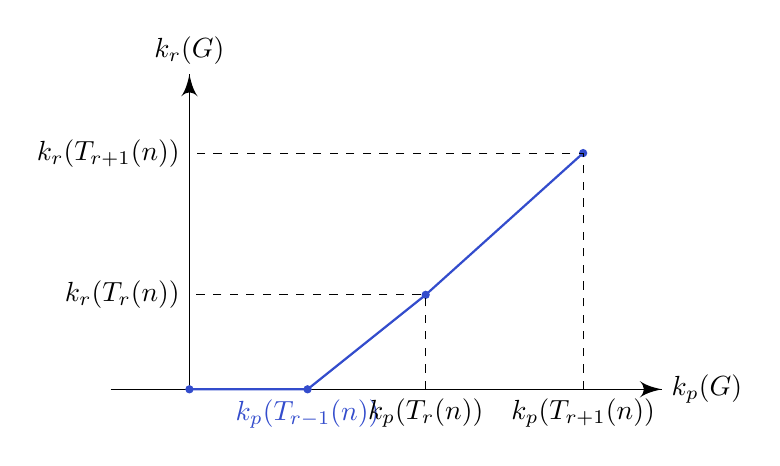
\begin{tikzpicture}
      \draw [->] (-1, 0) -- (6, 0) node [right] {$k_p(G)$};
      \draw [->] (0, 0) -- (0, 4) node [above] {$k_r(G)$};

      \draw [thick, mblue] (0, 0) node [circ] {} -- (1.5, 0) node [circ] {} node [below] {$k_p(T_{r - 1}(n))$} -- (3, 1.2) node [circ] {} -- (5, 3) node [circ] {};

      \draw [dashed] (3, 0) node [below] {$k_p(T_r(n))$} -- (3, 1.2) -- (0, 1.2) node [left] {$k_r(T_r(n))$};
      \draw [dashed] (5, 0) node [below] {$k_p(T_{r + 1}(n))$} -- (5, 3) -- (0, 3) node [left] {$k_r(T_{r + 1}(n))$};
    \end{tikzpicture}
  \end{center}
  The claim in the theorem is that if we go and plot $(k_p(G), k_r(G))$, then the point will be above the line. So suppose $G$ lies below $\psi$. Draw a straight line through the point parallel to $\psi$. This has slope $\frac{1}{c} > 0$ for some $c$. The intercept on the $x$-axis is then $k_p(G) - c k_r(G)$, which is greater than $f(\text{any Tur\'an graph})$.

  The previous theorem tells us $f$ is maximized on some complete multi-partite graph. Suppose this has $q$ class sizes, say $a_1 \leq a_2 \leq \cdots \leq a_q$. It is easy to verify $q \geq r - 1$. In fact, we may assume $q \geq r$, else the maximum is on a Tur\'an graph $T_{r - 1}(n)$.

  Then we have
  \[
    f(G) = a_1 a_q A - c a_q a_q B + C,
  \]
  where $A, B, C$ are rationals depending only on $a_2, \ldots, a_{q - 1}$ and $a_1 + a_q$ ($A$ and $B$ count the number of ways to pick a $K_p$ and $K_r$ respectively in a way that involves terms in both the first and last classes).

  We wlog assume $c$ is irrational. Hence $a_q a_q A - c a_1 a_q = a_1 a_q (A - cB) \not= 0$. If $A - cB < 0$, replace $a_1$ and $a_q$ by $0$ and $a_1 + a_q$. This would then increase $f$, which is impossible.

  If $A - cB > 0$ and $a_1 \leq a_q - 2$, then we can replace $a_1, a_q$ by $a_1 + 1, a_q - 1$ to increase $f$. Hence $a_1 \geq a_q - 1$. So $G = T_q(n)$.
\end{proof}

It was conjectured that the value of $\min \{k_3(G): e(G) = m, |G| = n\}$ is given by an $r$-partite graph, where $r$ is the minimum possible (subject to $e(G) = m$).

The continuous envelope of the conjection in range $\frac{1}{2}$ to $\frac{2}{3}$ was proved by Fisher in 1989. The whole range was proved (in the limit $n \to \infty$) was proved by Razborov in 2007, who introduced the method fof flag algebras. The idea was to use a computer to find the best possible Cauchy--Schwarz inequality, using semi-definite programming. Later in 2008, Nikiforov did $k_4$'s directly. Finally, Reiher did $k_r$'s for all $r$ by another method.

Finally, Liu, Pikhurko, Staden in 2017+ obtained the exact result for $k_3$'s (for $n$ large).

It is an open problem to maximize the number of induced paths of length $3$. We don't even have a conjecture.

\section{\texorpdfstring{Szemer\'edi's}{Szemeredi's} regularity lemma}
A graph with the (large scale) property that all subsets have the same density can be regarded as ``pseudo-random'' in a quantifiable sense. This lies behind the spirit of Szemer\'edi's lemma.

We look at bipartite graphs. Let $U, W$ be disjoint subsets of the vertex set of some graph. The number of edges between $U$ and $W$ is denoted by \term{$e(U, W)$}, and the density is
\[
  d(U, W) = \frac{e(U, W)}{|U| |W|}.
\]
\begin{defi}[$\varepsilon$-uniform pair]\index{$\varepsilon$-uniform}
  Let $0 < \varepsilon < 1$. We say a pair $(U, W)$ is \emph{$\varepsilon$-uniform} if
  \[
    |d(U', W') - d(U, W)| < \varepsilon
  \]
  whenever $U' \subseteq U$, $W' \subseteq W$, and $|U'| \geq \varepsilon |U|$, $|W'| \geq \varepsilon |W|$.
\end{defi}

Note that it is necessary to require impose some conditions on how $U'$ and $W'$ can be. For example, if $|U'| = |W'| = 1$, then $d(U', W')$ is either $0$ or $1$. So we cannot have a sensible definition if we want to require the inequality to hold for arbitrary $U', W'$.

But we might be worried that it is unnatural to use the same $\varepsilon$ for two different purposes. One can be reassured that the two uses are ``independent''. It is perfectly fine to use two separate parameters, but we will not do that for convenience.

First observe that an $\varepsilon$-uniform pair is roughly regular.
\begin{lemma}
  Let $(u, W)$ be an $\varepsilon$-uniform pair with $d(U, W) = d$. Then
  \begin{align*}
    |\{u \in U: |\Gamma(u) \cap W| > (d - \varepsilon) |W|\}| &\geq (1 - \varepsilon)|U|\\
    |\{u \in U: |\Gamma(u) \cap W| > (d + \varepsilon) |W|\}| &\geq (1 - \varepsilon)|U|,
  \end{align*}
  where $\Gamma(u)$ is the set of neighbours of $u$.
\end{lemma}
The proof is trivial. It is immediate from the definition.
\begin{proof}
  Let
  \[
    X = \{u \in U: |\Gamma(u) \cap W| \leq (d - \varepsilon)|W|\}.
  \]
  Then $e(X, W) \leq (d - \varepsilon) |X||W|$. So
  \[
    d(X, W) \leq d - \varepsilon = d(U, W) - \varepsilon.
  \]
  So it fails the uniformity condition. Since $W$ is definitely not small, we must have $|X| < \varepsilon |U|$.

  The other case is similar, or observe that the complementary bipartite graph between $U$ and $W$ has density $1 - d$ and is $\varepsilon$-uniform.
\end{proof}

We can use this idea repeatedly to build subgraphs.
\begin{lemma}
  Let $H$ be a graph with maximum degree $\Delta(H) \leq \Delta$. Suppose $H$ has an $r$-colouring so no colour is used more than $s$ times, i.e.\ $H \subseteq K_r(s)$. Let $G$ be a graph containing distinct vertex subsets $V_1, \ldots, V_r$ with $|V_i| = u$, such that $(V_i, V-j)$ is $\varepsilon$-uniform and $d(V_i, V_j) \geq \lambda$ for all $1 \leq i \leq j \leq r$.

  Suppose $(\Delta + 1) \varepsilon \leq \lambda^\Delta$ and $s \leq \lfloor \varepsilon u\rfloor$. Then $H \subseteq G$.
\end{lemma}

To prove this, we just do what we did in the previous lemma, and find lots of vertices connected to lots of other vertices, and then we are done.
\begin{proof}
  We wlog assume $V(H) = \{1, \ldots, k\}$, and let $c: V(H) \to \{1, \ldots, r\}$ be a colouring of $V(H)$ using no colour more than $s$ times. We'll pick vertices $x_1, \ldots, x_k$ in $G$ so that $x_i x_j \in E(G)$ if $ij \in E(H)$.

  We claim that, for $0 \leq \ell \leq k$, we can choose $x_1, \ldots, x_\ell$ so that $x_j \in C_{c(j)}$, and for $\ell < j \leq k$, there is a set $X^{\ell}_j$ of \emph{candidates} for $x_j$, satisfying $X_j^{\ell} \subseteq V_{c(j)}$, meaning is $x_i y_j \in E(G)$ for all $y_j \in X_j^{\ell}$ and $x_i \in N(j, \ell) = \{x_i: 1 \leq i \leq \ell \text{ and }ij \in E(H)\}$. Moreover, we claim we can do this so that
  \[
    |X_j^{\ell}| \geq (\lambda - \varepsilon)^{|N(j, \ell)|} |V_{c(j)}.
  \]

  The claim holds for $\ell = 0$ by taking $X_j^0 = V_{c(j)}$.

  In general, for each $t \in T = \{j > \ell + 1 : (\ell + 1)j \in E(H)\}$, we let
  \[
    Y_t =  \{y \in X_{\ell + 1}^{\ell} : |\Gamma(y) \cap X_t^\ell| \leq (\lambda - \varepsilon) |X^{\ell}_t|\}.
  \]
  Let $m = |N(\ell + 1, \ell)|$. Note that $m + |T| \leq \Delta$.

  Since
  \[
    d(Y_t, X_{\ell + 1}^\ell) \leq \lambda - \varepsilon \leq d(V_{c(t)}, V_{c(\ell + 1)}) - \varepsilon,
  \]
  and
  \[
    |X_{\ell + 1}| \geq (\lambda - \varepsilon)^{\Delta - 1} |V_{c(t)}| \geq (\lambda^{\Delta - 1} - (\Delta - 1)\varepsilon) |V_{c(t)}| > \varepsilon |V_{c(t)}|.,
  \]
  we have
  \[
    |Y_t \leq \varepsilon |V_{c(\ell + 1)}|.
  \]
  Therefore
  \[
    \left|X_{\ell + 1}^{\ell} - \bigcup_{t \in T} Y_t \right| \geq (\lambda - \varepsilon)^m |V_{c(\ell + 1)}| - (\Delta - m) \varepsilon|V_{c(\ell + 1)}| \geq (\lambda^m - m\varepsilon - (\Delta - m)\varepsilon) u \geq \varepsilon u > s - 1.
  \]
  At most $s - 1$ vertices of $X_{\ell + 1}^\ell - \bigcup Y_t$ have been chosen amongst $x_1, \ldots, x_\ell$, so we may select $x_{\ell + 1}$ in this set. Then take
  \[
    X^{\ell + 1}_t = X^\ell_t \cap \Gamma(x_{\ell + 1})
  \]
  for $t \in T$, and for $t \not \in T$, we just set $X_j^{\ell + 1} X_j^{\ell}$.

  This establishes the claim for $1 \leq \ell \leq k$, completing the proof.
\end{proof}

\begin{cor}
  Let $H$ be a graph with vertex set $\{v_1, \ldots, v_k\}$. Let $0 < \lambda, \eta < 1$ satisfy $k \eta \leq \lambda^{k - 1}$. Let $G$ be a graph with disjoint vertex subsets $V_1, \ldots, V_k$, each of size $u \geq 1$. Suppose each pair $(V_i, V_j)$ is $\eta$ uniform, and $d(V_i, V_j) \geq \lambda$ if $v_i v_j \in E(H)$, and $d(V_i, V_j) \leq 1 - \lambda$ if $v_i v_j \not \in E(H)$. Then there exists $x_i \in V_i$, so the map $v_i \to x_i$ is an isomorphism $H \to G[\{x_1, \ldots, x_k\}]$.
\end{cor}

\begin{proof}
  By replacing the $V_i$-$V_j$ edges by the complementary set whenever $v_i v_j \not \in E(H)$, we may assume $d(V_i, V_j) \geq \lambda$ for all $i, j$, and $H$ is a complete graph.

  We then apply the previous lemma by taking $\varepsilon = \eta$, $r = k$, $\Delta = k- 1$ and $s = 1$.
\end{proof}

Remarkably, Szemer\'edi showed that every graph can be partitioned into finitely many classes, most pairs being $\varepsilon$-uniform.

An \term{equipartition} of $v(G)$ into $k$ parts is a partition into sets $V_1, \ldots, V_k$, where $\lfloor \frac{n}{k} \rfloor \leq V_i \leq \lceil n/k\rceil$, where $n = |G|$.

We say that the partition is $\varepsilon$-uniform\index{$\varepsilon$-uniform!partition} if $(V_i, V_j)$ is $\varepsilon$-uniform for all but $\varepsilon \binom{k}{2}$ pairs.

\begin{thm}[Szemer\'edi's regularity lemma]\index{Szemer\'edi regularity lemma}
  Let $0 < \varepsilon < 1$ and let $\ell$ be some natural number. Then there exists some $L = L(\ell, \varepsilon)$ such that every graph has an $\varepsilon$-uniform equipartition into $m$ parts for some $\ell \leq m \leq L$, depending on the graph.
\end{thm}
This lemma was proved by Szemer\'edi in order to prove his theorem on arithmetic progressions in dense subsets of integers.

When we want to apply this, we usually want at least $\ell$ many prats. For example, having $1$ part is usually not very helpful. The upper bound on $m$ is helpful for us to ensure the parts are large enough, by picking graphs with sufficiently many vertices.

We first need a couple of trivial lemmas.
\begin{lemma}
  Let $U' \subseteq U$ and $W" \subseteq W$, where $|U'| \geq (1 - \delta)|U|$ and $|W'| \geq (1 - \delta) |W|$. Then
  \[
    |d(U', W') - d(U, W)| \leq 2\delta.
  \]
\end{lemma}

\begin{proof}
  Let $d = d(U, W)$ and $d' = d(U', W')$. Then
  \[
    d = \frac{e(U, W)}{|U||W|} \geq \frac{e(U', W')}{|U||W|} = d' \frac{|U'||W'|}{|U||W|} \geq d' (1 - \delta)^2.
  \]
  Thus,
  \[
    d' - d \leq d'(1 - (1 - \delta)^2) \leq 2d d' \leq 2 \delta.
  \]
  The other inequality follows from considering the complementary graph, which tells us
  \[
    (1 - d') - (1 - d) \leq 2\delta.
  \]
\end{proof}

\begin{lemma}
  Let $x_1, \ldots, x_n$ be real numbers with
  \[
    X = \frac{1}{n} \sum_{i = 1}^n x_i,
  \]
  and let
  \[
    x = \frac{1}{m} \sum_{i = 1}^m x_i.
  \]
  Then
  \[
    \frac{1}{n} \sum_{i = 1}^n x_i^2 \geq X^2 + \frac{m}{n - m}(x - X)^2 \geq X^2 + \frac{m}{n} (x - X)^2.
  \]
\end{lemma}<++>
If we ignore the second term on the right, then this is just Cauchy--Schwarz.

\begin{proof}
  We have
  \begin{align*}
    \frac{1}{n} \sum_{i = 1}^n x_i^2 &= \frac{1}{n} \sum_{i = 1}^m x_i^2 + \frac{1}{n} \sum_{i = m + 1}^n x_i^2 \\
    &\geq \frac{m}{n} x^2 + \frac{n - m}{n} \left(\frac{nX - mx}{n - m}\right)^2\\
    ^\geq X^2 + \frac{m}{n - m} (x - X)^2
  \end{align*}
  by two applications of Cauchy--Schwarz.
\end{proof}

We can now prove Szemer\'edi's regularity lemma.
\begin{proof}
  Define the index $\ind(\mathcal{P})$ of an equipartition $\mathcal{P}$ into $k$ parts $V_i$ to be
  \[
    \ind(P) = \frac{1}{k^2} \sum_{i < j} d^2(V_i, V_j).
  \]
  We show that if $P$ is not $\varepsilon$-uniform, then there is a refinement equipartition $\mathcal{Q}$ into $k 4^k$ parts, with $\ind(\mathcal{Q}) \geq \ind(\mathcal{P}) + \frac{\varepsilon^5}{8}$.

  This is enough to prove the theorem. For choose $t \geq \ell$ with $4^t \varepsilon^5 \geq 100$. Define recursively a function $f$ by
  \[
    f(0) = t,\quad f(j + 1) = f(j) 4^{f(j)}.
  \]
  Let
  \[
    N = f(\lceil 4 \varepsilon^{-5}\rceil),
  \]
  and pick $L = N 16^N$.

  Then, if $n \leq L$, then just take an equipartition into single vertices. Otherwise, begin with a partition into $t$ parts. As long as the current partition into $k$ parts is not $\varepsilon$ uniform, replace it a refinement into $4 k^4$ parts. The point is that $\ind(\mathcal{P}) \leq \frac{1}{2}$ for any partition. So we can't do this more than $4 \varepsilon^{-5}$ times, at which point we have partitioned into $N \leq L$ parts.

  Note that the reason we had to set $L = N 16^N$ is that in our proof, we want to assume we have many vertices lying around.

  The proof really is just one line, but students tend to complain about such short proofs, so let's try to explain it in a bit more detail. If the partition is not $\varepsilon$-uniform, this means we can further partition each part into uneven pieces. Then our previous lemma tells us this discrepancy allows us to push up $\frac{1}{n} \sum x_i^2$.

  So given an equipartition $\mathcal{P}$ that is not $\varepsilon$-uniform, for each non-uniform pair $(V_i, V_j)$ of $P$, we pick witness sets
  \[
    X_{ij} \subseteq V_i,\quad X_{ji} \subseteq V_j
  \]
  with $|X_{ij}| \geq \varepsilon |V_i|$, $|X_{ji}| \geq |V_j|$ and $|d(X_{ij}, X_{ji}) - D(V_i, V_j)| \geq \varepsilon$.

  Fix $i$. Then the sets $X_{ij}$ partition $V_i$ into at most $2^{k - 1}$ \term{atoms}. Let $m = \lfloor\frac{n}{k4^k}\rfloor$, and let $n = k 4^k m + ak + b$, where $0 \leq a \leq 4^k$ and $b \leq k$. Then we see that
  \[
    \lfloor n/k\rfloor = 4^k m + a
  \]
  and the parts of $\mathcal{P}$ have size $4^k m + a$ or $4^km + a + 1$, with $b$ of the larger size.

  Partition each part of $\mathcal{P}$ into $4^k$ sets, of size $m$ or $m + 1$. The smaller $V_i$ having $a$ parts of size $m + 1$, and thelargrer having $a + 1$ such pairs.

  We see that any such partition is an equipartition into $k 4^k$ parts of size $m$ or $m + 1$, with $ak + b$ parts of larger size $m + 1$.

  Let's choose such an equipartition $\mathcal{Q}$ with parts as nearly as possible inside atoms, so each atom is a union of parts of $\mathcal{Q}$ with at most $m$ extra vertices.

  All that remains is to check that $\ind (\mathcal{Q}) \geq \ind(\mathcal{P}) + \frac{\varepsilon^5}{8}$.

  Let the sets of $\mathcal{Q}$ within $V_i$ be $V_i(s)$, where $1 \leq s \leq 4^k \equiv q$. So
  \[
    V_i = \bigcup_{s = 1}^q V_i(s).
  \]
  Now
  \[
    \sum_{1 \leq s, t \leq q} e(V_i(s), V_j(t)) = e(V_i, V_j).
  \]
  We'd like to divide by some numbers and convert these to densities, but this is where we have to watch out. But this is still quite easy to handle. We have
  \[
    \frac{m}{m + 1} \leq q |V_i(s)| \leq |V_i| \leq \frac{m + 1}{m} q |V_i(s)|
  \]
  for all $s$. So we want $m$ to be large for this to not hurt us too much.

  So
  \[
    \left(\frac{m}{m + 1}\right) d(V_i, V_j) \leq \frac{1}{q^2} \sum_{s, t} d(V_i(s), V_j(t)) \leq \left(\frac{m + 1}{m}\right)^2 d(V_i, V_j).
  \]
  Using $n \geq k 16^k$, and hence
  \[
    \left(\frac{m}{m + 1}\right)^2 \geq  1 - \frac{2}{m} \geq 1 - \frac{2}{4^k} \geq 1 - \frac{\varepsilon^5}{50},
  \]
  we have
  \[
    \left|\frac{1}{q^2} \sum_{s, t} d(V_i(s), V_j(t)) - d(V_, V_j)\right| \leq \frac{\varepsilon^5}{49} + d(V_i, V_j). % s/49/50/ ?
  \]
  In particular,
  \[
    \frac{1}{q^2} \sum d^2(V_i(s), V_j(t)) \geq d^2(V_i, V_j) - \frac{\varepsilon^5}{25}.
  \]
  The lower bound can be improved if $(V_i, V_j)$ is not $\varepsilon$-uniform.

  Let $X_{ij}^*$ be the largest subset of $X_{ij}$ that is the union of parts of $\mathcal{Q}$. We may assume
  \[
    X_{ij}^* = \bigcup_{1 \leq s \leq r_i} V_i(s).
  \]
  By an argument similar to the above, we have
  \[
    \frac{1}{r_i r_j} \sum_{1 \leq s \leq r_i, 1 \leq t \leq r_j} d(V_i(s), d_j(t)) \leq d(X_{ij}^*, X_{ji}^*) + \frac{\varepsilon^5}{49}.
  \]
  By the choice of parts of $\mathcal{Q}$ within atoms, and because $|V_i| \geq qm = 4^k m$, we have
  \begin{align*}
    |X_{ij}^*| &\geq |X_{ij}| - 2^{k - 1}m \\
    &\geq |X_{ij}| (1 - \frac{2^k m}{\varepsilon |V_i|}) \\
    &\geq |X_{ij}| \left(1 - \frac{1}{2^k \varepsilon}\right)\\
    &\geq |X_{ij}| \left(1 - \frac{\varepsilon}{10}\right).
  \end{align*}
  So by the lemma, we know
  \[
    |d(X_{ij}^*, X_{ji}^*) - d(X_{ij}, X_{ji})| < \frac{\varepsilon}{5}.
  \]
  Recalling that
  \[
    |d(X_{ij}, X_{ji}) - d(V_i, V_j)| > \varepsilon,
  \]
  we have
  \[
    \left| \frac{1}{r_i r_j} \sum_{1 \leq s \leq r_i, 1 \leq t \leq r_j} d(V_i(s), V_j(t)) - d(V_i, V_j)\right| > \frac{3}{4} \varepsilon.
  \]
  We can now allow our Cauchy--Schwarz inequality with $n = q^2$ and $m = r_i r_j$ gives
  \begin{align*}
    \frac{1}{q^2} \sum_{1 \leq s, t \leq q} d^2 (V_i(s), V_j(t)) &\geq d^2(V_i, V_j) - \frac{\varepsilon^5}{25} + \frac{r_i r_j}{q^2}\cdot \frac{9\varepsilon^2}{16} \\
    &\geq d^2(V_i, V_j) - \frac{\varepsilon^5}{25} + \frac{\varepsilon^4}{3},
  \end{align*}
  using the fact that
  \[
    \frac{r_i}{q} \geq \left(1 - \frac{1}{m}\right) \frac{r_i}{q} \frac{m + 1}{m} \geq \left(1 - \frac{1}{m}\right) \geq \frac{|X_{ij}^*|}{|V_i|} \geq \left(1 - \frac{1}{m}\right) \left(1 - \frac{\varepsilon}{10}\right) \frac{|X_{ij}|}{|V_i|} > \frac{4\varepsilon}{5}.
  \]
  Therefore
  \begin{align*}
    \ind(\mathcal{Q}) &= \frac{1}{k^2q^2}\sum_{1 \leq i < j < k; 1 \leq s, t\leq q} d^2(V_i(s), V_j(t))\\
    &\geq \frac{1}{k^2} \sum_{1 \leq i < j \leq k} d^2(V_i, V_j) - \frac{\varepsilon^5}{25} + \varepsilon \binom{k}{2} \frac{\varepsilon^4}{3}\\
    &\geq \ind(P) + \frac{\varepsilon^5}{8}.\qedhere
  \end{align*}
\end{proof}
The proof gives something like
\[
  L \sim 2^{2^{.^{.^{.^{2}}}}},
\]
where the tower is $\varepsilon^{-5}$ tall. Can we do better than that?

In 1997, Gowers showed that the tower of height at least $\varepsilon^{-1/16}$. Indeed, define $V_1, \ldots, V_k$ to be $(\varepsilon, \delta, \eta)$-uniform if all but $\eta \binom{k}{2}$ pairs $(V_i, V_j)$ satisfy $|d(V_i, V_j) - d(V_i', V_j')| \leq \varepsilon$ whenever $|V_i'| \geq \delta |V_i|$. Then the graph for which every $(1 - \delta^{1/16}, \delta, 1 - 20 \delta^{1/16})$-uniform partition needs a tower height $\delta^{-1/16}$ parts.

More recently, Moskowitz and Shapira (2012) improved these bounds. Most recently, a reformulation of the lemma due to Lov\'asz and Szegedy (2007) for which the upper bound is tower($\varepsilon^{-2}$) was shown to have lower bound tower($\varepsilon^{-2}$) by Fox and Lov\'asz (2014) (note that these are different Lov\'asz's!).

Let's now look at some applications of the Szemer\'edi's regularity lemma. Recall that Ramsey's theorem says there exists $R(k)$ so every red-blue colouring of the edges of $K_n$ yeidls a monochromatic $K_k$ provided $n \geq R(k)$. There are known bounds
\[
  2^{k/2} \leq R(k) \leq 4^k.
\]
The existence of $R(k)$ implies that for every graph $G$, there exists a number $r(G)$ minimal so if $n \geq r(G)$ and we colour $K_n$, we obtain a monochromatic $G$. Clearly, we have
\[
  r(G) \leq R(|G|).
\]
How much smaller can $r(G)$ be compared to $R(|G|)$?

\begin{thm}
  Given an integer $d$, there exists $c(d)$ such that
  \[
    r(G) \leq c|G|
  \]
  for every graph $G$ with $\Delta(G) \leq d$.
\end{thm}

\begin{proof}
  Let $t = R(d + 1)$. Pick $\varepsilon \leq \min \left\{\frac{1}{t}, \frac{1}{2^d (d + 1)}\right\}$. Let $\ell \geq t^2$, and let $L = L(\ell, \varepsilon)$. We show that $c = \frac{L}{\varepsilon}$ works.

  Indeed, let $G$ be a graph. Colour the edges of $K_n$ by red and blue, where $n \geq c |G|$. Apply Szemir\'edi to the red graph with $\ell, \varepsilon$ as above. Let $H$ be the graph whose vertices are $\{V_1, \ldots, V_m\}$, where $V_1, \ldots, V_m$ is the partition of the red graph. Let $V_i, V_j \in E(H)$ if $(V_i, V_j)$ is $\varepsilon$-uniform. Notice that $m = |H| \geq \ell \geq t^2$, and $e(\bar{H}) \leq \varepsilon \binom{m}{2}$. So $H \supseteq K_t$, or else by Tur\'an's theroem, there are integers $d_1, \ldots, d_{t - 1}$ and $\sum d_i m$ and
  \[
    e(\bar{H}) \geq \binom{d_i}{2}\geq (t - 1) \binom{m/(t - 1)}{2} \geq \varepsilon \binom{m}{2}
  \]
  by our choice of $\varepsilon$ and $m$.
\end{proof}

\printindex
\end{document}
